%%%%%%%%%%%%%%%%%%%%%%%%%%%%%%%%%%%%%%%%%%%%%%%%%%%%%%%%%%%%%%%%%%%%
%%%%% HEADER %%%%%
%%%%%%%%%%%%%%%%%%%%%%%%%%%%%%%%%%%%%%%%%%%%%%%%%%%%%%%%%%%%%%%%%%%%

\documentclass[a4paper]{article}


%%%%% Packages %%%%%

	%%%%% Language %%%%% 
\usepackage[frenchb]{babel}
\usepackage[utf8]{inputenc}
\usepackage[T1]{fontenc}
	%%%%% Graphic %%%%%
\usepackage{graphicx}
	%%%%% Mise en page %%%%%
\usepackage{fancyhdr}
	%%%%% Tableaux %%%%%
\usepackage{colortbl} 

%%%%% Macros %%%%
\newcommand{\HRule}{\rule{\linewidth}{0.5mm}}

\pagestyle{fancy}
\lhead{EMF Project \\ Projet de Vérification et tests}
\rhead{Coraline \textsc{Marie} \\ Vincent \textsc{Raveneau}}

%%%%% Doc's informations %%%%%


%%%%%%%%%%%%%%%%%%%%%%%%%%%%%%%%%%%%%%%%%%%%%%%%%%%%%%%%%%%%%%%%%%%%
%%%%% DOCUMENT %%%%%
%%%%%%%%%%%%%%%%%%%%%%%%%%%%%%%%%%%%%%%%%%%%%%%%%%%%%%%%%%%%%%%%%%%%

\begin{document}

	%%%%% Page de garde %%%%
	\begin{titlepage}
		\begin{center}

			
\includegraphics[width=0.45\textwidth]{UN-sciences.png}~\\[2cm]

			\LARGE{Master 1 \sc{Alma}}\\[1.5cm]

			\Large{Projet de Vérification et tests}\\[0.5cm]

			% Titre
			\HRule \\[0.4cm]
			{ \huge \bfseries EMF Project \\[0.4cm] }
			\HRule \\[1.5cm]

			% Auteur et Encadrant
			\normalsize		
			\emph{\'Etudiants :}\\
			Coraline \textsc{Marie} et Vincent \textsc{Raveneau}\\
			\vspace{0.5cm}
			\emph{Intervenant :} \\
			Gerson \textsc{Sunyé}
		
			\vfill

			% Bottom of the page
			{\large 13 décembre 2013}

		\end{center}
	\end{titlepage}


	%%%%% Sommaire %%%%%
	\renewcommand{\contentsname}{Sommaire}
	\tableofcontents
	\newpage


	%%%%% Introduction %%%%%
	\begin{center}
		\section{Introduction}
	\end{center}

	\vspace{0.5cm}

	La création d'un logiciel, quel qu'il soit, n'est jamais sûre. Le code source peut contenir des fautes, des bugs ou des défauts, sans même que le programmeur ne les remarque. Fort heureusement, il existe aujourd'hui des méthodes efficaces pour contrer ces failles, et renforcer la fiabilité du code source, comme par exemple les tests unitaires.

	\vspace{0.5cm}

	Le module \textit{Vérification et Tests} que nous avons étudié en Master \textsc{Alma} à l’Université de Nantes, nous a apporté un ensemble de techniques utilisables sur la majorité des langages informatique. Pour parfaire cet apprentissage, nous avons travaillé sur la restructuration et l'amélioration de l'EMF (Eclipse Modeling Framework), un logiciel libre développé pour et par Eclipse.

	\vspace{0.5cm}

	Ce rapport présente donc une application directe de ce que nous a appris le module Vérification et tests, au travers de deux grandes étapes de travail. Pour la première, nous avons tout d'abord dû restructurer une partie du code source de l'EMF en un projet Maven. Puis nous avons dû évaluer les tests déjà présent dans ce code. Pour la seconde étape nous avons dû améliorer autant que possible la qualité de la classe URI, afin d'augmenter sa fiabilité.

	\newpage


	%%%%% Partie 1 %%%%%
	\begin{center}
		\section{Restructuration et évaluation}
	\end{center}

	\vspace{0.5cm}

		%%%%% Partie 1.1 %%%%%
		\subsection{Réorganisation avec Maven}

		\vspace{0.5cm}

		L'un des objectifs pédagogiques du projet de vérification et tests, était de nous apprendre à utiliser un nouvel outil : Maven. 

		\subsubsection{Qu'est ce que Maven ?}

		\vspace{0.5cm}

		Maven (ou Apache Maven) est un logiciel libre, qui permet la gestion et la production automatique de projets liés au langage de programmation Java. Il s'agit d'un outil, qui aide à la conception de logiciels à partir du code source, en optimisant les tâches et en garantissant le bon ordre de fabrication.

		\vspace{0.5cm}

		\subsubsection{Conversion du code original}

		\vspace{0.5cm}

		Le code source original du projet EMF est disponible sur gitHub. Il est donc téléchargeable en archive, et modifiable par n'importe qui. Cependant, l'archive que nous avons récupérée fournit un code source conditionné pour l'environnement de développement Eclipse, et cet IDE nous a été fortement déconseillé.

		\vspace{0.5cm}

		Ainsi, pour répondre à la demande du cahier des charges de ne pas utiliser Eclipse, nous avons choisi un nouvel IDE compatible avec Maven pour travailler. Ce choix s'est porté sur l'IDE NetBeans, qui permet de supporter plusieurs langages, et possédant un plugin de gestion de Maven. Cependant, le code source original devait être au préalable adapté, avant de pouvoir le travailler.

		\vspace{0.5cm}

		Afin d'optimiser notre travail, nous n'avons pas converti la totalité de l'archive téléchargée, mais juste la partie du code intéressante pour le projet. Malgré la facilité de conversion de l'architecture, cette tâche fût relativement fastidieuse. Certaines erreurs de package et de plugin sont apparues, ce qui nous a pris du temps à résoudre. De plus, tous les tests du projet étant mis dans un unique dossier, il nous a fallu identifier ceux qui étaient liés au code sur lequel nous avions à travailler.

		\vspace{0.5cm}

		Voici l'arborescence obtenue après la conversion du code source original en projet Netbeans/Maven : 

		\begin{center}
			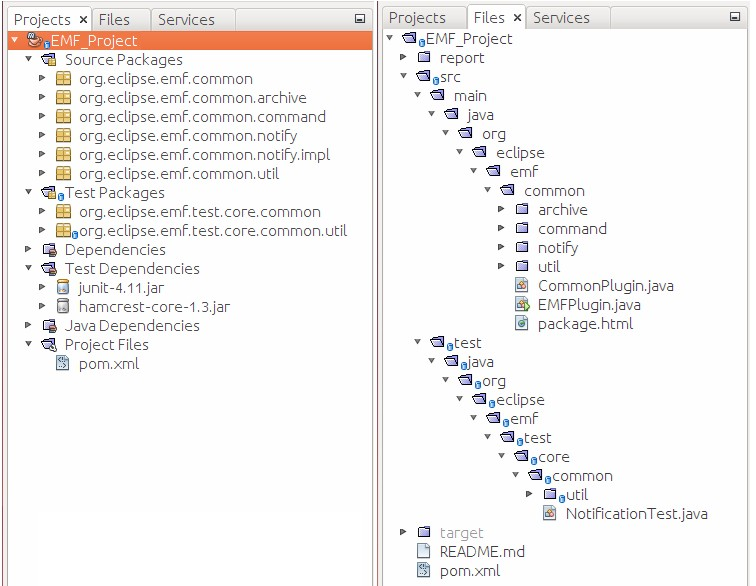
\includegraphics[width=1.0\textwidth]{Arborescence.jpg}~\\
		\end{center}

		\vspace{0.5cm}

		\subsubsection{Bugs et résolution}

		\vspace{0.5cm}

		Pour gérer les bibliothèques et les dépendances d'un projet, Maven utilise un fichier \texttt{pom.xml}, qui décrit l'ensemble des besoins de l'application. Lors de la conversion du code source initial vers notre projet Maven, plusieurs erreurs liées à ce fichier sont apparues, car il manquait des dépendances :
		\begin{itemize}
			\item JUnit : framework de test unitaire.
			\item Core Runtime : framework (de Eclipse RCP).
			\item EMF ecore et EMF ecore xmi.
		\end{itemize}

		\vspace{0.5cm}



		%%%%% Partie 1.2 %%%%%
		\subsection{Passage des tests à JUnit 4.11}

		\vspace{0.5cm}

		Il a d'abord été nécessaire de mettre les tests existants à jour, afin qu'ils puissent être exécutés par la version 4.11 de JUnit. En effet, ceux ci étaient basés sur une version obsolète de JUnit. Cette partie n'a pas demandé énormément de travail, étant donné qu'elle a principalement consisté à supprimer les inclusions de l'ancienne version de JUnit afin de les remplacer par les récentes. Il a également été nécessaire de rajouter l'annotation \texttt{@Test} avant chaque méthode de test unitaire, afin que l'appel à JUnit puisse les identifier clairement.

		%%%%%% Partie 1.3 %%%%%%%%
		\subsection{Evaluation de la qualité des tests}

		\vspace{0.5cm}

		Afin d'évaluer la qualité des tests présents, nous avons procédé en trois étapes:

		\subsubsection{Exécution des tests}

		\vspace{0.5cm}

		Nous avons tout d'abord exécuté les tests, afin de voir s'ils échouaient ou réussissaient, ainsi que leur nombre.

		Comme le montre l'image suivante, les 23 tests exécutés sont tous positifs, ce qui est une bonne chose.

		\begin{center}
			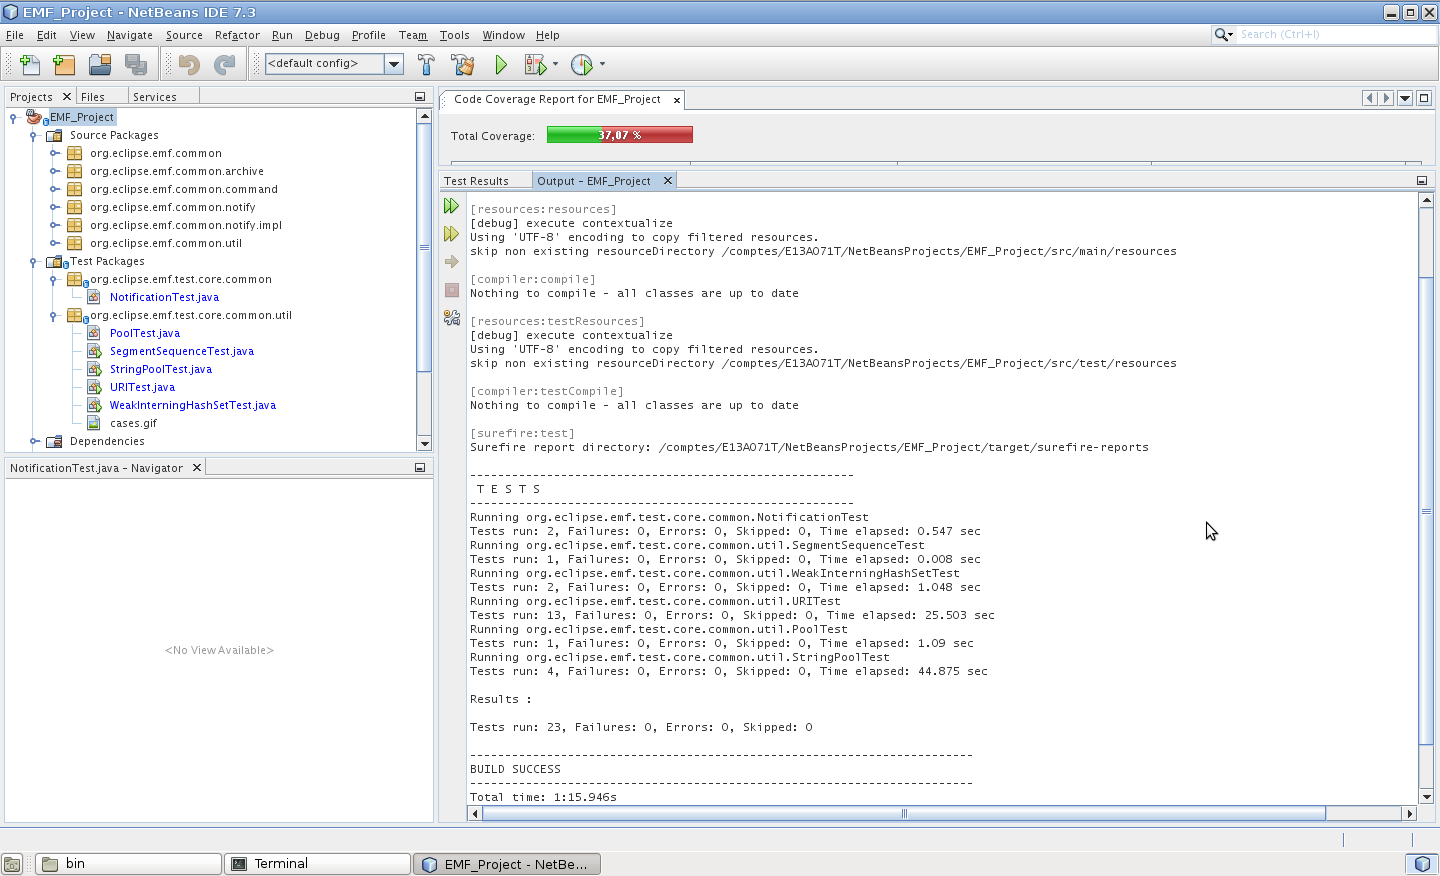
\includegraphics[width=1.0\textwidth]{tests_execution.png}~\\
		\end{center}

		\subsubsection{Couverture du code}

		\vspace{0.5cm}

		Nous avons ensuite utilisé Cobertura, un outils de couverture de code permettant de mettre en évidence la proportion du code effectivement exécutée lors de l'appel des tests unitaires.

		Comme le montre l'image suivante, uniquement 37\% du code est testé. Même si ce pourcentage est faible, il est intéressant de remarquer que la majorité des classes sont soit complètement couvertes, soit pas du tout (très peu de classes ont une couverture partielle).

		\begin{center}
			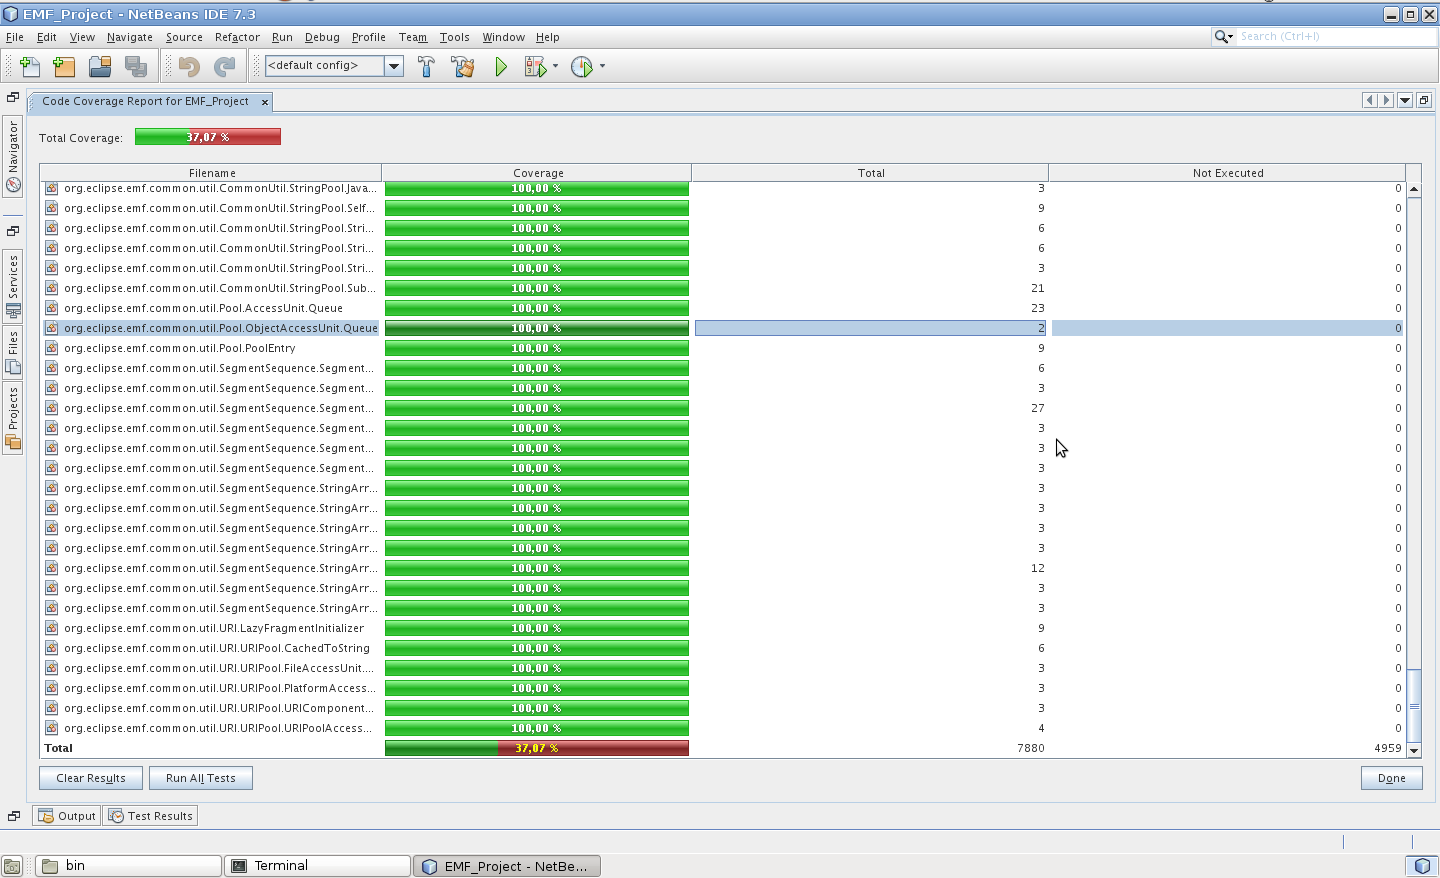
\includegraphics[width=1.0\textwidth]{couverture.png}~\\
		\end{center}

		\subsubsection{Analyse de mutation}

		\vspace{0.5cm}

		Nous avons enfin utilisé Pit, un outils d'analyse de mutation. Il permet de générer des mutants afin de tester si de légères modifications du code permettent de tromper la suite de tests, ou s'ils sont détectés.

		Malheureusement, très peu de ces mutants sont détectés, et la majorité des rapports d'exécution de Pit sont similaires à celui présent sur l'image suivante.

		\begin{center}
			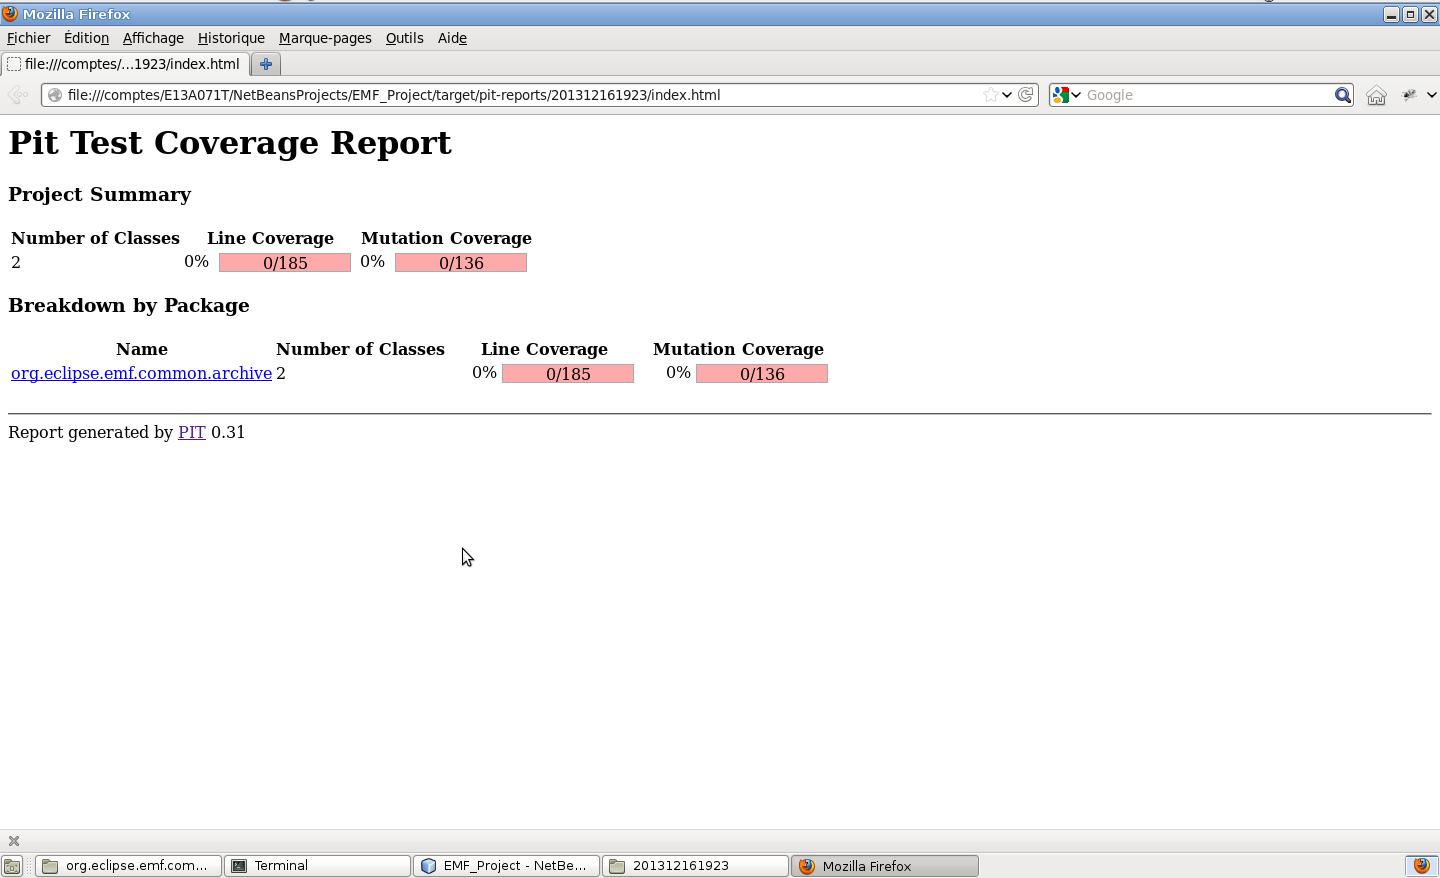
\includegraphics[width=1.0\textwidth]{CapturePit.png}~\\
		\end{center}

		%%%%%%%%% Partie 1.4 %%%%%%%%%%%
		\subsection{Conclusion sur la partie 1}

		Suite à ces observations, on peut conclure que la suite de tests actuellement présente sur le projet n'est ni exhaustive (elle est même très loin de l'être au vu des résultats de couverture du code), ni vraiment efficace, comme le montrent les résultats de l'analyse de mutation. Il est donc nécessaire d'améliorer celle-ci, d'une part en étendant la couverture effectuée, et d'autre part en implémentant plus de cas de test afin de mieux identifier les erreurs induites par les mutants.

	\newpage

	%%%%% Partie 2 %%%%%
	\begin{center}
		\section{Amélioration de URI}
	\end{center}

	\vspace{0.5cm}

	Il nous était ensuite demander de travailler sur une unique classe, la classe URI du package \texttt{org/eclipse/emf/common/util}, afin d'améliorer sa qualité, ainsi que celle de ses tests. Malheureusement, nous n'avons pas pu effectuer cette partie, faute de temps.

		\vspace{0.5cm}

		%%%%% Partie 2.1 %%%%%
		\subsection{La classe URI}

		\vspace{0.5cm}

			Après avoir terminé la première partie du projet, c'est à dire réorganiser le dossier pour Maven et réparer les erreurs de compatibilités, nous avons chercher les défauts de conceptions de la classe URI. Malheureusement nous avons manqué de temps pour mener à bien cette étape, et nous n'avons pas trouvé de défaut pertinent pour la suite de notre travail. Cette classe n'a donc pas été modifiée.

			\newpage

	\begin{center}
		\section{Conclusion}
	\end{center}	
		Bien que nous n'ayons pas totalement terminé ce travail, le projet de Vérification et Tests reste un projet d'apprentissage. Nous avons appris de nouvelles notions, comme l'utilisation de Maven et de son système d'architecture. Nous avons également amélioré nos compétences en informatique en travaillant sur le code d'autres programmeurs, et en le retravaillant.

		\vspace{0.5cm}

		Ce projet nous a permis d'utiliser nos nouvelles connaissances étudiées en \textit{Vérification et Tests}, mais pas seulement. Nous nous sommes servis pour ce projet d'autres notions vues dans d'autres modules d'enseignement, comme par exemple \textit{Concepts et Outils de Développement}, ou \textit{Génie Logiciel}.
 
\end{document}
